\documentclass[10pt,pdf]{beamer}
\usepackage[utf8]{inputenc}
\usepackage[russian]{babel}

\usepackage{beamerthemesplit}
\usetheme[numbers, minimal, nonav, nologo]{Statmod}
\setbeamertemplate{caption}[numbered]
\setbeamertemplate{blocks}[rounded]
\setbeamertemplate{title page}[default][colsep=-4bp,rounded=true]
\setbeamertemplate{frametitle}[default][colsep=-4bp,rounded=true]
\setbeamercolor{normal text}{fg=black}
\setbeamercolor*{structure}{fg=black,bg=white}
\setbeamercolor*{palette primary}{use=structure,fg=black,bg=structure.bg}
\setbeamercolor*{palette secondary}{use=structure,fg=black,bg=structure.bg}
\setbeamercolor*{palette tertiary}{use=structure,fg=black,bg=structure.bg}
\setbeamerfont{footline}{series=\normalfont\small}
\setbeamersize{text margin left=5mm, text margin right=5mm}

\date{Волгоград, 2014}
\title{Модификация уравнения Нернста--Планка для пассивного транспорта}
\author{Абдрахманов В. Л., гр. Ф-469}
\institute{Руководитель --- профессор, д.ф.-м.н. Шеин А. Г.}

\newcommand{\pder}[2] {\frac{\partial #1}{\partial #2}}
\newcommand{\ppder}[2]{\frac{\partial^2 #1}{\partial {#2}^2}}
\newcommand{\pcder}[3]{\frac{\partial^2 #1}{\partial #2 \partial #3}}
\newcommand{\der}[2]  {\frac{d #1}{d #2}}
\newcommand{\dder}[2] {\frac{d^2 #1}{d {#2}^2}}

\newcommand{\const}{\mathrm{const}}
\newcommand{\average}[1]{\left\langle #1 \right\rangle}
\newcommand{\abs}[1]{\left| #1 \right|}
\newcommand{\ds}{\displaystyle}
\newcommand{\D}{\Delta}
\newcommand{\dotunder}[1]{\d{#1}}
\renewcommand{\d}{\delta}
\newcommand{\eps}{\varepsilon}
\renewcommand{\phi}{\varphi}

\newcommand{\divergence}{\mathrm{div\,}}
\newcommand{\gradient}  {\mathrm{grad\,}}
\newcommand{\rotor}     {\mathrm{rot\,}}

\begin{document}
  \frame{\titlepage}
  \begin{frame}
    \frametitle{Введение}

    \textbf{Актуальность.} Наличие высокочастотных полей в настоящее 
    время является постоянным фактором, поэтому изучение их влияния
    на живой организм необходимо. Создание моделей, позволяющих описать
    воздействие СВЧ-излучения на мембранный транспорт
    хотя бы с учетом ограничений и приближений, является актуальной
    задачей.
    \vspace*{2em}

    \textbf{Цель работы} заключается в получении уравнений, описывающих
    влияние высокочастотных полей на ионные токи в мембранах. При
    рассмотрении задачи ионного транспорта в электродиффузионном подходе
    используется уравнение Нернста—Планка, которое применимо в
    стационарном случае, то есть когда ток постоянен. Так как 
    электрические колебания --- нестационарный процесс, то необходимо 
    модифицировать уравнение для нестационарного случая.
\end{frame}
  \begin{frame}
    \frametitle{Уравнение Нернста--Планка}
    \begin{figure}[H]
        \center
        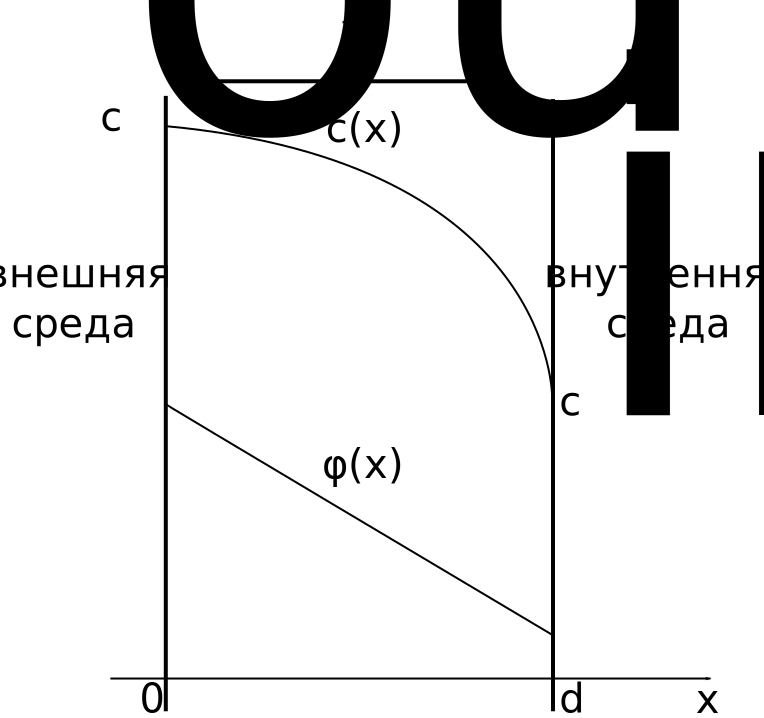
\includegraphics[height=.5\textheight]{membrane}
    \end{figure}
    \begin{equation}
        j = -\frac{z}{\abs{z}}uRT\pder{c}{x} -
        \abs{z}ucF\pder{\phi}{x}.
        \label{eq:nernst-plank}
    \end{equation}
  \end{frame}
  \begin{frame}
      \begin{minipage}{.47\textwidth}
      Приближённое решение Планка
    \begingroup
    \everymath{\scriptstyle}
    \scriptsize
      \begin{equation}
          c(x) = \chi x + c(0),\ \chi = \frac{c(d)-c(0)}{d},
      \end{equation}
      \begin{equation}
          \phi(x) = \phi(0)
          -\frac{\phi_0}{\ln[c(d) / c(0)]}\ln\frac{\chi x + c(0)}{c(0)}.
      \end{equation}
      \endgroup
      \begin{figure}[H]
          \center
          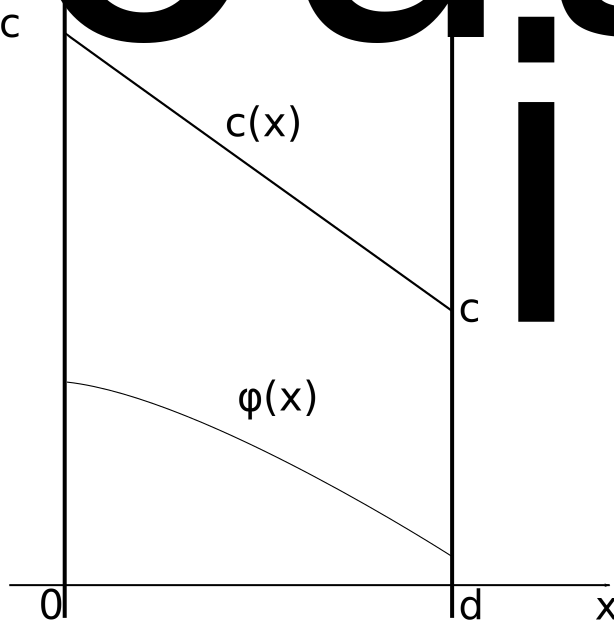
\includegraphics[height=.5\textheight]{planck}
      \end{figure}
      \end{minipage}\hfill
      \begin{minipage}{.47\textwidth}
      Приближённое решение Гольдмана
    \begingroup
    \everymath{\scriptstyle}
    \scriptsize
      \begin{equation}
          \phi(x) = \phi(0) - Ex, E = \frac{\phi_0}{d},
      \end{equation}
      \begin{equation}
          c(x) = c(0) + [c(d) - c(0)]
          \frac{e^{\alpha x} - 1}{e^{\alpha d} - 1},
          \alpha = \frac{zFE}{RT}.
      \end{equation}
      \endgroup
      \begin{figure}[H]
          \center
          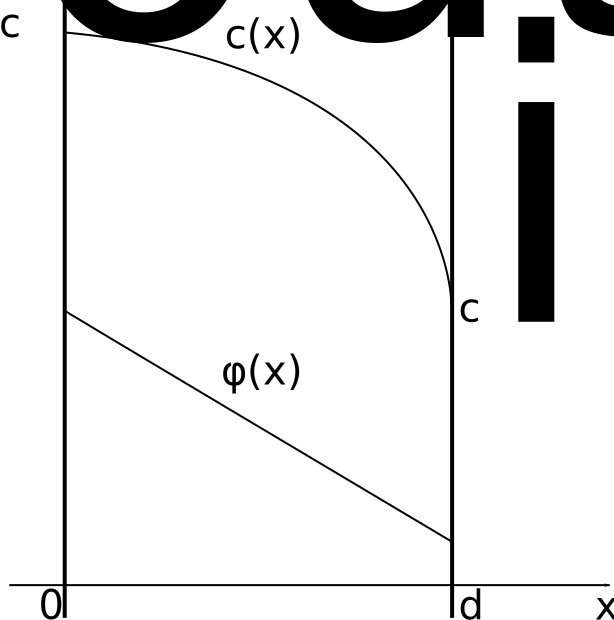
\includegraphics[height=.5\textheight]{goldman}
      \end{figure}
    \end{minipage}
  \end{frame}
  \begin{frame}
      \frametitle{Нестационарное уравнение}
        \begin{equation}
          j = -\frac{z}{|z|}uRT\pder{c}{x} - |z|ucF\pder{\phi}{x}.
        \end{equation}
        \begin{equation}
            \pder{\rho}{t} + \divergence\vec{j} = 0.
        \end{equation}
        Учитывая, что \( \rho = zcF \), получим уравнение
        \begin{equation}
            \pder{c}{t} = D\ppder{c}{x} +
            \frac{z}{|z|}u\pder{\phi}{x}\pder{c}{x} +
            \frac{z}{|z|}u\ppder{\phi}{x}c,\quad D = \frac{uRT}{F|z|}.
        \end{equation}
  \end{frame}
  \begin{frame}
      \frametitle{Решение для планковского и гольдмановского приближений}

      \begin{minipage}{.47\textwidth}
      Планковское приближение
          \begingroup
\everymath{\scriptstyle}
\scriptsize
        \begin{align*}
        & \pder{c}{\tau} = \ppder{c}{\xi} - wg(\xi)\pder{c}{\xi} + wg^2(\xi)c,
            \ \xi\in(0,1) \\
        & \tau = \frac{D}{d^2}t,\ \xi = \frac{x}{d},\ w = \frac{vd}{D},
        \ g(\xi) = \frac{1}{\xi - \frac{c_{out}}{c_{out} - c_{in}}},\\
        & c(0, \tau) = c_{out},\ \tau>0 \\
        & c(1, \tau) = c_{in},\ \tau>0 \\
        & c(\xi, 0) = 0,\ \xi\in(0,1).
    \end{align*}
\endgroup
\end{minipage}\hfill
      \begin{minipage}{.47\textwidth}
      Гольдмановское приближение
\begingroup
\everymath{\scriptstyle}
\scriptsize
        \begin{align*}
            & \pder{c}{\tau} = \ppder{c}{\xi} -
                w\pder{c}{\xi},\ \xi\in(0,1) \\
            & \tau = \frac{D}{d^2}t,\ \xi = \frac{x}{d},\ w = \frac{vd}{D},\\
            & c(0, \tau) = c_{out},\ \tau>0 \\
            & c(1, \tau) = c_{in},\ \tau>0 \\
            & c(\xi, 0) = 0,\ \xi\in(0,1).
        \end{align*}
\endgroup
    \end{minipage}\hfill
\end{frame}
\begin{frame}
    \begin{figure}[H]
    \begin{center}
        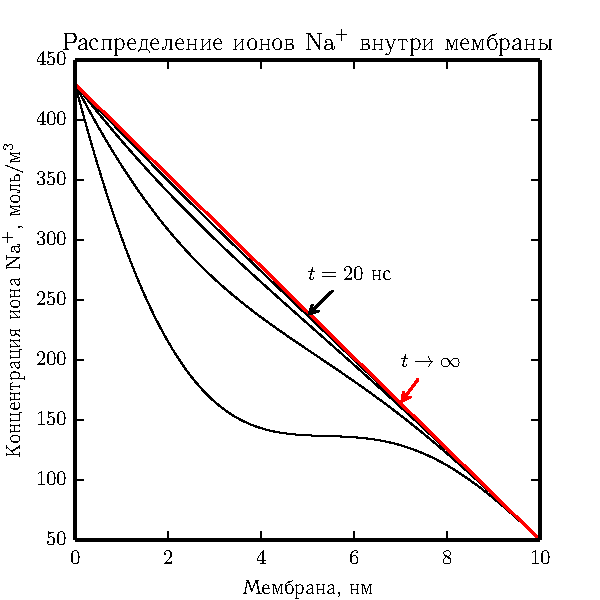
\includegraphics[width=.47\textwidth]{../plots/linear_conc}
    \hfill
        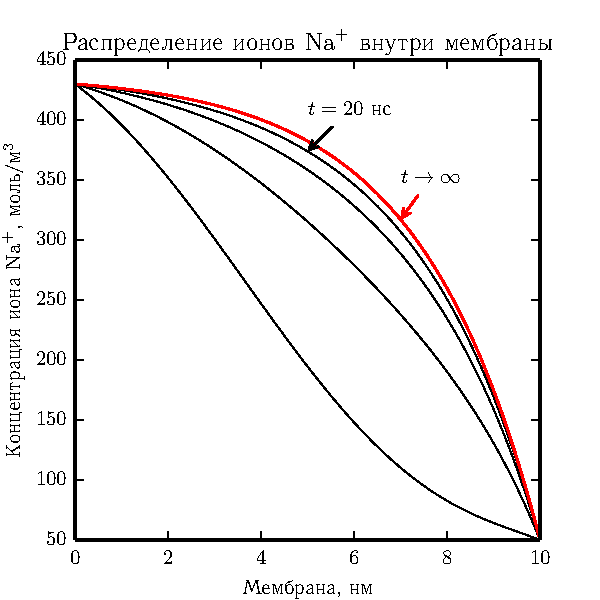
\includegraphics[width=.47\textwidth]{../plots/linear_field}
    \end{center}
    \end{figure}


  \end{frame}
  \begin{frame}
      \frametitle{Учёт уравнения Пуассона}
      \begin{equation}
        \pder{E}{x} = \frac{cFz}{\eps\eps_0},\quad
        c = \frac{\eps\eps_0}{Fz}\pder{E}{x}.
    \end{equation}
    \begin{equation}
        j = \eps\eps_0
            \left(-D\ppder{E}{x}+\frac{z}{|z|}uE\pder{E}{x}\right).
        \label{eq:j_from_E}
    \end{equation}
    \begin{equation}
        \pder{\rho}{t} + \pder{j}{x} = 0.
    \end{equation}
    \begin{equation}
        \pder{j}{x} = -\eps\eps_0\pcder{E}{x}{t}.
        \label{eq:displacement-current}
    \end{equation}
    \begin{equation}
        \pcder{E}{x}{t} = D\frac{\partial^3{E}}{\partial x^3} -
        \frac{z}{\abs{z}}\frac{u}{2}\ppder{E^2}{x}.
        \label{eq:epic-equation}
    \end{equation}
    Граничное условие
    \begin{equation}
        \left.\pder{E}{x}\right|_{x=0} = \frac{Fz}{\eps\eps_0}c(0),\quad
        \left.\pder{E}{x}\right|_{x=d} = \frac{Fz}{\eps\eps_0}c(d).
    \end{equation}
    \end{frame}
  \begin{frame}
    \frametitle{Добавление СВЧ-поля}
    \[
        E_m << E^{(0)}
    \]
    \begin{equation}
        E = \underbrace{E_m e^{i\omega t}}_\text{возмущение} +
        \underbrace{E^{(0)}}_\text{стационарное поле} +
        E^{(1)} + \ldots.
    \end{equation}
    \begin{gather}
    \pcder{E^{(1)}}{x}{t} = D\frac{\partial^3 E^{(1)}}{\partial x^3} +
    \frac{uzE^{(0)}}{\abs{z}}\ppder{E^{(1)}}{x} +
    2\frac{uz}{\abs{z}}\pder{E^{(0)}}{x}\pder{E^{(1)}}{x} +\nonumber \\+
    \frac{uz}{\abs{z}}\ppder{E^{(0)}}{x} E^{(1)} +
    \frac{uz}{\abs{z}}\ppder{E^{(0)}}{x} E_m e^{i\omega t}.
\end{gather}
  \end{frame}
  \begin{frame}
      \frametitle{Заключение}
      В данной работе предпринята попытка получить эквивалент уравнения
Нернста—Планка для нестационарного процесса. Получено уравнение, которое может быть использовано для рассмотрения нестационарного
процесса переноса ионов в мембране, однако его недостатком является то,
что для его решения требуется явный вид профиля потенциала в мембране. В
качестве попытки обойти эту проблему, было получено уравнение,
которое включает в себя только одну неизвестную функцию. Но и это
уравнение в том виде, в котором оно получено, не может решить
поставленную задачу, так как для постановки краевой задачи требуется 3
граничных условия, в то время как у нас имеется только 2. Тем не менее,
если удастся решить эту проблему, то данное уравнение можно будет
использовать для описания транспорта ионов в мембране при наличии
высокочастотного поля.
  \end{frame}
\end{document}
